\section{Experiments and results}


\subsection{Custom CNN: Training and results}


The training phase for the custom CNN baseline is designed to evaluate the architecture's ability to learn discriminative features directly from the raw data. In contrast to subsequent experiments, this model is trained \textbf{from scratch}, with all weights initialized randomly. The optimization process seeks to minimize the standard \textbf{Cross-Entropy Loss}: $$\mathcal{L} = -\frac{1}{N} \sum_{i=1}^{N} \sum_{c=1}^{C} y_{i,c} \log(\hat{y}_{i,c})$$
where $C=101$ represents the action classes of the UCF101 dataset.\\\\
We employ the \textbf{Adam optimizer} with a fixed learning rate of $\eta = 10^{-3}$ to ensure a stable convergence during the 50 epochs.\\\\
To ensure the selection of the most generalizable parameters, we implement a strict \textbf{Model Checkpointing} policy: the model state is saved only when a new peak in validation accuracy is recorded. Furthermore, an \textbf{Early Stopping} mechanism is employed to prevent the model from over-fitting once the performance floor is reached. Training is prematurely terminated if the validation loss fails to decrease by a minimum threshold of $0.001$ for \textbf{10 consecutive epochs}.\\\\
The data pipeline is managed through an optimized \texttt{DataLoader} with a \textbf{Batch Size} of 32, and \textbf{shuffling} enabled to prevent the model from learning the specific order of samples within the dataset splits.


\begin{figure}[h]
    \centering
    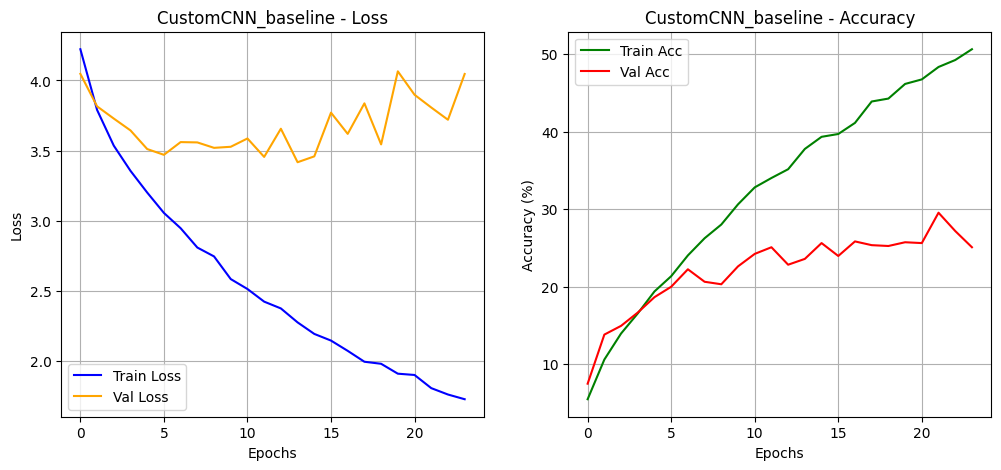
\includegraphics[width=1\textwidth]{images/perf1.png}
    \caption{Training and Validation Performance of Custom CNN.}
    \label{fig:custom_cnn_perf}
\end{figure}
\noindent
The experimental results of the Custom CNN ~\ref{fig:custom_cnn_perf} reveal a sharp divergence between training and validation metrics occurring as early as the fifth epoch. This trend indicates that the network, due to its shallow architecture and the absence of pre-trained weights, quickly exhausts its representational capacity. Instead of learning generalizable action patterns, the model begins to memorize the training data noise, leading to severe overfitting.\\\\
A final test accuracy of 27.76\% provides quantitative evidence that the dataset and the task’s complexity substantially exceed the model’s capacity, making it inadequate for reliable action recognition. In essence, this outcome underlines the necessity of transitioning from a \textit{"proof-of-concept"} scratch-trained model to a more advanced, deeper architecture that leverages the benefits of transfer learning.



\subsection{ResNet18 with temporal mean pooling: Training and results}

\begin{itemize}
    \item \textbf{Fine-tuning Strategy}: Adaptation of ResNet18 to the UCF101 dataset, preserving pre-trained spatial features.
    \item \textbf{Optimization}: Categorical Cross-Entropy loss paired with the Adam optimizer.
    \item \textbf{Learning Rate}: $\eta = 10^{-5}$ for a maximum of 50 epochs, ensuring conservative weight updates.
    \item \textbf{Validation Policies}: Model Checkpointing and Early Stopping with a patience of 10 epochs ($\Delta = 0.001$).
    \item \textbf{Data Pipeline}: Optimized batch size of 32 with data shuffling.
\end{itemize}

\begin{table}[h]
\centering
\caption{Top 5 Worst and Best Performing Classes}
\label{tab:class_accuracy_extremes}
\begin{tabular}{l c @{\quad} l c}
\toprule
\multicolumn{2}{c}{\textbf{Most Difficult Classes}} &
\multicolumn{2}{c}{\textbf{Best Performing Classes}} \\
\cmidrule(r){1-2} \cmidrule(l){3-4}
\textbf{Class Name} & \textbf{Accuracy (\%)} &
\textbf{Class Name} & \textbf{Accuracy (\%)} \\
\midrule
HandstandWalking & 0.00  & SumoWrestling     & 100.00 \\
JumpRope         & 2.63  & Skijet            & 100.00 \\
BodyWeightSquats & 10.00 & Surfing           & 100.00 \\
Nunchucks        & 11.43 & Rafting           & 100.00 \\
WallPushups      & 20.00 & VolleyballSpiking & 100.00 \\
\bottomrule
\end{tabular}
\end{table}

\begin{figure}[h]
    \centering
    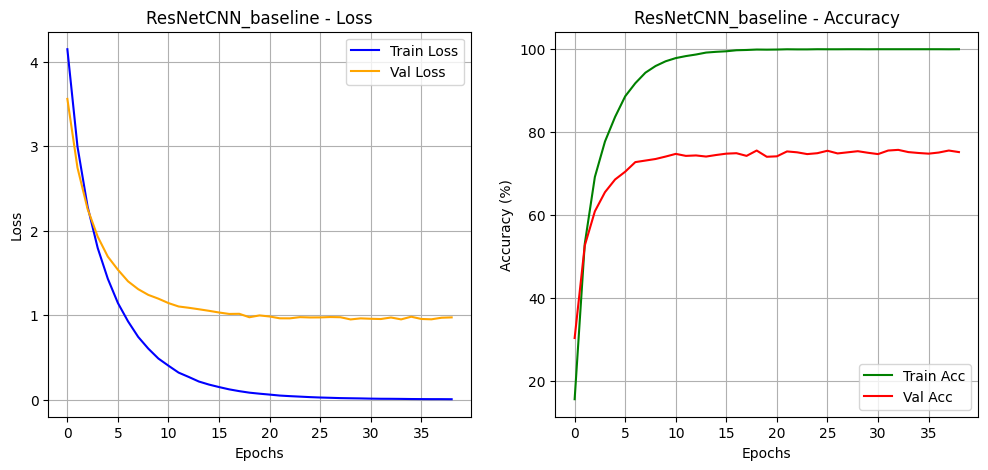
\includegraphics[width=1\textwidth]{images/perf2.png}
    \caption{Training and Validation Performance of ResNet18 with Temporal Mean Pooling.}
    \label{fig:custom_cnn_perf2}
\end{figure}

\noindent
As shown in Figure~\ref{fig:custom_cnn_perf2}, the transition to a ResNet18 backbone yields a 75.71\% test accuracy. However, the model fails on purely dynamic actions such as \textit{HandstandWalking} (0\%) and \textit{JumpRope} (2.63\%) (Table~\ref{tab:class_accuracy_extremes}). Because the \textit{Bag-of-Frames} approach collapses the temporal dimension, the architecture remains a scene classifier unable to distinguish motion-dependent patterns. This "temporal collapse" justifies the transition to a sequential architecture to capture the missing dynamics.




\subsection{ResNet18 with LSTM: Training and results}

The training process for the ResNet-LSTM architecture utilizes several advanced strategies to optimize the end-to-end fine-tuning:

\begin{itemize}
    \item \textbf{Differential Learning Rates}: We employ the \textbf{AdamW} optimizer with a weight decay of $10^{-4}$. To balance feature preservation and temporal adaptation, the backbone uses $\eta = 10^{-5}$, while the LSTM and classifier modules use $\eta = 10^{-4}$.
    \item \textbf{Label Smoothing}: The cross-entropy loss incorporates a \textbf{label smoothing} factor of $0.1$ to improve generalization and prevent the model from becoming overconfident on the complex UCF101 samples.
    \item \textbf{Learning Rate Scheduling}: A \textbf{ReduceLROnPlateau} scheduler is implemented, reducing the learning rate by a factor of $0.1$ if the validation loss plateaus for $7$ consecutive epochs.
    \item \textbf{Convergence Control}: Given the increased complexity of the recurrent module, the early stopping \textbf{patience} is extended to $15$ epochs (with a delta of $0.001$) to allow for stable convergence.
\end{itemize}


\begin{figure}[h]
    \centering
    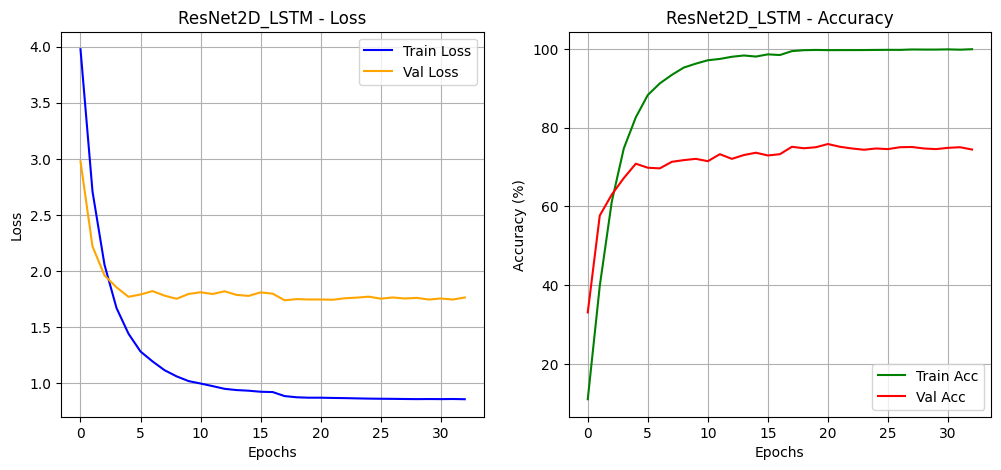
\includegraphics[width=1\textwidth]{images/perf3.png}
    \caption{Training and Validation Performance of ResNet18+LSTM.}
    \label{fig:cnn_perf3}
\end{figure}

\noindent
The results of the training and validation in figure~\ref{fig:cnn_perf3} show that the model has a very high learning capacity, reaching 100\% training accuracy quickly. However, the gap between training and validation loss is wider than in the simple ResNet baseline, suggesting that adding an LSTM makes the model more complex and prone to overfitting.\\\\
The test results shown that the final accuracy is 73.88\%, a slight decrease from the 75.71\% of the previous ResNet-only model. However, the table of class extremes shows a vital improvement in dynamic actions:
\begin{itemize}
    \item \textbf{Action Recognition}: Purely dynamic classes are finally recognized. \textit{HandstandWalking} jumped from 0\% to \textbf{20.59\%}, proving the LSTM is capturing temporal patterns previously ignored.
    \item \textbf{Static Backgrounds}: Top-performing classes remain at \textbf{100\% accuracy}, as the ResNet backbone easily identifies their unique visual environments.
    \item \textbf{Unidirectional Limits}: Classes with fast, repetitive motions like \textit{JumpRope} (5.26\%), \textit{Nunchucks} (11.43\%), \textit{YoYo} (13.89\%) remain difficult.
\end{itemize}

\begin{table}[h]
\centering
\caption{Top 5 Worst and Best Performing Classes with ResNet18+LSTM}
\label{tab:class_accuracy_extremes_updated}
\begin{tabular}{l c @{\quad} l c}
\toprule
\multicolumn{2}{c}{\textbf{Most Difficult Classes}} &
\multicolumn{2}{c}{\textbf{Best Performing Classes}} \\
\cmidrule(r){1-2} \cmidrule(l){3-4}
\textbf{Class Name} & \textbf{Accuracy (\%)} &
\textbf{Class Name} & \textbf{Accuracy (\%)} \\
\midrule
JumpRope          & 5.26  & PlayingFlute  & 100.00 \\
Nunchucks         & 11.43 & Diving        & 100.00 \\
YoYo              & 13.89 & PlayingViolin & 100.00 \\
HandstandWalking  & 20.59 & Rowing        & 100.00 \\
BrushingTeeth     & 27.78 & Surfing       & 100.00 \\
\bottomrule
\end{tabular}
\end{table}


\subsection{ResNet18 with BiLSTM: Training and results}
The ResNet18-BiLSTM architecture represents a significant evolution in our temporal modeling, utilizing a bidirectional approach to capture dependencies from both the past and future states of a sequence. The training strategy is detailed below:

\begin{itemize}
    \item \textbf{Differential Learning Rates}: To ensure stable end-to-end fine-tuning, we employ the \textbf{AdamW} optimizer with a weight decay of $10^{-4}$. We apply a stratified learning rate strategy: the ResNet18 backbone is tuned with $\eta = 10^{-5}$ to preserve pretrained spatial features, while the BiLSTM and the MLP classifier use $\eta = 10^{-4}$.
    \item \textbf{Robust Regularization}: Beyond the standard \textbf{Label Smoothing} ($0.1$), we implement a multi-stage dropout strategy. This includes \textbf{Spatial Dropout} ($0.6$) on the extracted features and specific dropout layers within the BiLSTM ($0.5$) and the final classifier to mitigate overfitting on the UCF101 dataset.
    \item \textbf{Gradient Management}: To prevent gradient explosions common in deep recurrent networks, we apply \textbf{Gradient Clipping} with a maximum norm of $1.0$.
    \item \textbf{Optimization Scheduling}: We utilize the \textbf{ReduceLROnPlateau} scheduler, which monitors the validation loss and reduces the learning rate by a factor of $0.1$ after $7$ epochs of stagnation. The training is governed by an \textbf{Early Stopping} policy with a patience of $15$ epochs to ensure the model reaches its optimal generalization point.
\end{itemize}


\begin{figure}[h]
    \centering
    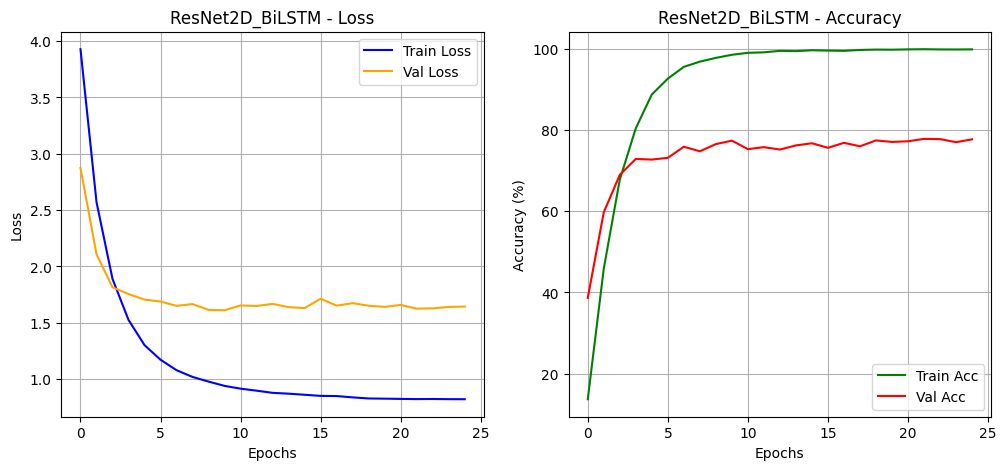
\includegraphics[width=1\textwidth]{images/perf4.png}
    \caption{Training and Validation Performance of ResNet18+BiLSTM.}
    \label{fig:cnn_perf4}
\end{figure}

\noindent
As shown in Figure \ref{fig:cnn_perf4}, the model exhibits rapid convergence, with training accuracy reaching near-saturation within 15 epochs. While a gap between training and validation performance suggests a degree of overfitting, the stability of the validation loss indicates successful regularization through spatial dropout ($0.6$) and weight decay.\\\\
The ResNet18-BiLSTM model achieved a final test accuracy of \textbf{78.14\%}, demonstrating a significant improvement (+7.04\%) over the original RGB-only LRCN baseline of 71.1\%. The results provide deep insights into the model's ability to synthesize temporal information.\\\\
The classification performance reveals a clear distinction between actions:
\begin{itemize}
    \item \textbf{Top Performers}: Classes such as \textit{PlayingPiano}, \textit{Typing}, and \textit{Surfing} achieved \textbf{100\% accuracy}. These categories benefit from strong spatial cues and consistent environmental backgrounds that the ResNet18 backbone identifies with high confidence.
    \item \textbf{Failure Cases and Temporal Gain}: The model lowest scores represent a measurable improvement over previously models. This suggests that the BiLSTM is extracting motion cues that were previously inaccessible. This transition from static scene recognition to dynamic action understanding confirms that the recurrent layers are effectively modeling the chronological evolution of the sequences, even in high-ambiguity scenarios.
\end{itemize}

\begin{table}[h]
\centering
\caption{Top 5 Worst and Best Performing Classes on the Test Set}
\label{tab:final_class_accuracy_extremes}
\begin{tabular}{l c @{\quad} l c}
\toprule
\multicolumn{2}{c}{\textbf{Most Difficult Classes}} &
\multicolumn{2}{c}{\textbf{Best Performing Classes}} \\
\cmidrule(r){1-2} \cmidrule(l){3-4}
\textbf{Class Name} & \textbf{Accuracy (\%)} &
\textbf{Class Name} & \textbf{Accuracy (\%)} \\
\midrule
HandstandWalking & 17.65 & PlayingPiano & 100.00 \\
JumpRope         & 26.32 & Surfing      & 100.00 \\
CricketShot      & 28.57 & Skijet       & 100.00 \\
Nunchucks        & 37.14 & Rowing       & 100.00 \\
BodyWeightSquats & 40.00 & Typing       & 100.00 \\
\bottomrule
\end{tabular}
\end{table}

\subsection{Transformer VideoMAE: Training and Results}

The fine-tuning of the VideoMAE architecture utilizes a high-capacity Transformer backbone, specifically the \texttt{videomae-base} variant, which benefits from extensive self-supervised pre-training on the Kinetics-400 dataset for 1,600 epochs \cite{Tong2022}. To adapt this "Masked Autoencoder" for the supervised classification task on UCF101, we implemented the following protocol:

\begin{itemize}
    \item \textbf{Input Pipeline and Dimensionality}: The model processes clips of 16 frames with a resolution of $224 \times 224$. Unlike convolutional models, we applied a dimension \textbf{permutation} to the input tensor, shifting the temporal dimension before the color channels $(B, T, C, H, W)$ to satisfy the Transformer's attention mechanism requirements.
    \item \textbf{Optimization Strategy}: We utilized the \textbf{AdamW} optimizer with a conservative learning rate of $\eta = 5 \times 10^{-5}$. This choice prevents the massive pre-trained weights from being "washed away" by large gradients during the initial epochs, focusing instead on stabilizing the newly initialized classification head.
    \item \textbf{Loss and Regularization}: To mitigate the high risk of overfitting associated with Vision Transformers (ViT) on medium-sized datasets, we employed \textbf{Cross-Entropy Loss with Label Smoothing} ($0.1$). This encourages the model to be less overconfident, facilitating better generalization during the transfer learning process.
    \item \textbf{Inference Constraints}: To maintain a focus on computational efficiency and real-time applicability, we adopted a \textbf{single-view inference} strategy, processing only the central clip of each video rather than the computationally expensive multi-view approach typically seen in literature \cite{Tong2022}.
\end{itemize}


\begin{figure}[h]
    \centering
    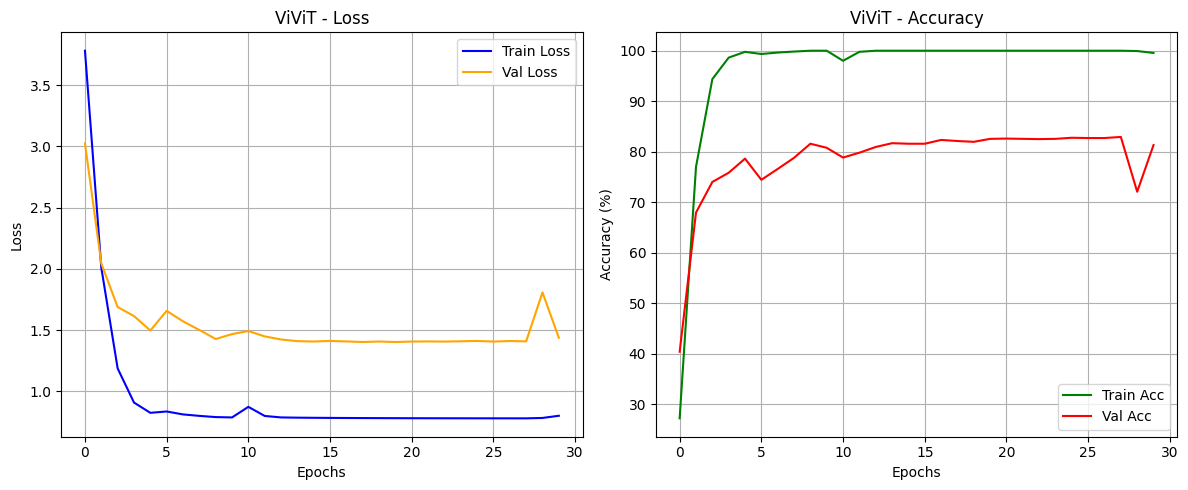
\includegraphics[width=1\textwidth]{images/perf5.png}
    \caption{Training and Validation Performance of fine-tuned VideoMAE-base.}
    \label{fig:cnn_perf5}
\end{figure}

The VideoMAE-base model achieved a peak validation accuracy of \textbf{82.92\%}, establishing itself as the superior architecture in our comparative study. However, the training dynamics reveal a profound "generalization gap" that warrants technical discussion.


\begin{itemize}
    \item \textbf{Rapid Convergence}: The model reached $100\%$ training accuracy by Epoch 9. This suggests that the self-supervised pre-training on Kinetics-400 provided such rich spatiotemporal features that the model effectively "memorized" the UCF101 training distribution almost instantly \cite{Tong2022}.
    \item \textbf{Performance Delta}: Despite the overfitting, VideoMAE outperformed the ResNet18-BiLSTM baseline by $+4.62\%$. This confirms that global self-attention mechanisms are inherently better at capturing the complex dynamics of actions like \textit{CricketShot} or \textit{JumpRope} compared to recurrent hidden states.
    \item \textbf{Saturation and Plateau}: The stagnation of the validation loss around $1.40$ indicates that without advanced data augmentation (e.g., Mixup or RandAugment), the model's high capacity leads to a representational bottleneck where further training only reinforces existing biases rather than discovering new discriminative features \cite{Tong2022}.
\end{itemize}

\subsubsection{Addressing the Gap with State-of-the-Art Benchmarks}
It is important to contextualize our result of $82.92\%$ against the published SOTA of $96.1\%$ for VideoMAE on UCF101 \cite{Tong2022}. This discrepancy is not indicative of architectural failure, but rather of the simplified evaluation protocol adopted for this study:

\begin{enumerate}
    \item \textbf{Inference Protocol}: SOTA benchmarks utilize \textbf{multi-view testing}, typically averaging predictions over 12 views (3 temporal clips $\times$ 4 spatial crops) per video \cite{Tong2022}. Our study employs a single-view, single-crop inference to prioritize real-time feasibility.
    \item \textbf{Data Augmentation}: Official results rely on heavy regularization techniques such as \textit{Mixup}, \textit{CutMix}, and \textit{RandAugment}, which are essential to prevent Transformers from overfitting on smaller datasets like UCF101.
    \item \textbf{Supervised Pre-training}: While our model uses self-supervised weights, SOTA results often start from checkpoints already fine-tuned on the full Kinetics-400 labels, providing a more discriminative starting point.
\end{enumerate}

The final evaluation on the test set yielded an accuracy of \textbf{79.0\%} for the VideoMAE model. While this represents a marginal improvement of \textbf{+1\%} over the ResNet18-BiLSTM baseline (78\%), the results suggest that both architectures encounter a similar performance ceiling when constrained to single-view inference and a 16-frame temporal window. \\
As illustrated in Table \ref{tab:worst5_classes_final}, the classes that pose the greatest challenge remain largely consistent across both modeling paradigms. 

\begin{table}[h]
\centering
\caption{Top 5 Most Difficult Classes on the Test Set}
\label{tab:worst5_classes_final}
\begin{tabular}{l c}
\toprule
\textbf{Class Name} & \textbf{Accuracy (\%)} \\
\midrule
BrushingTeeth     & 11.11 \\
HandstandWalking  & 20.59 \\
Nunchucks         & 22.86 \\
ShavingBeard      & 30.23 \\
Hammering         & 30.30 \\
\bottomrule
\end{tabular}
\end{table}

\noindent
In conclusion, without advanced data augmentation or multi-crop evaluation, the latent representational power of the Transformer cannot fully compensate for the lack of high-frequency spatial details.